%% 由 build/emit_tex.py 生成（生成物，勿手改）；定制请放 user_style.tex / user_meta.yaml
\chapter{第 1 章 ·
复数和复平面}\label{ux7b2c-1-ux7ae0-ux590dux6570ux548cux590dux5e73ux9762}

\section{1.1 复数}\label{ux590dux6570}

\begin{quote}
本节目标：理解复数的代数形式、几何表示、模与辐角，能熟练进行复数的四则运算、乘方与开方，并掌握复数的三角形式、指数形式及其几何意义。
重点：模与辐角、乘除法的几何意义、n 次方根。 难点：辐角的多值性、主值
arg z 的确定。
\end{quote}

\subsection{1.1.1 复数的概念}\label{ux590dux6570ux7684ux6982ux5ff5}

\textbf{定义 1.1} 形如

\[
z = a + ib,\qquad a,b \in \mathbb{R}
\]

的数称为复数，其中 \(i\) 称为\textbf{虚单位}，满足

\[
i^2 = -1 .
\]

\(a\) 与 \(b\) 分别称为复数 \(z\) 的实部和虚部，记作

\[
a = \operatorname{Re} z,\qquad b = \operatorname{Im} z .
\]

\begin{itemize}
\tightlist
\item
  当且仅当 \(b=0\) 时，\(z=a\) 是实数；
\item
  当且仅当 \(a=b=0\) 时，\(z\) 就是实数 \(0\)；
\item
  当 \(b\neq 0\) 时，\(z\) 称为\textbf{虚数}；
\item
  当 \(a=0\) 且 \(b\neq 0\) 时，\(z=ib\) 称为\textbf{纯虚数}。
\end{itemize}

全体复数组成的集合称为\textbf{复数集}，记作 \(\mathbb{C}\)；实数集
\(\mathbb{R}\) 是 \(\mathbb{C}\) 的真子集。

两个复数 \(z_1=a+ib\) 与 \(z_2=c+id\)
相等，当且仅当它们的实部和虚部分别相等：

\[
z_1 = z_2 \iff a=c \ \text{且}\ b=d .
\]

\subsection{1.1.2
复数的几何表示与复平面}\label{ux590dux6570ux7684ux51e0ux4f55ux8868ux793aux4e0eux590dux5e73ux9762}

复数 \(z=a+ib\) 可用平面上的点 \(z(a,b)\)
表示。用直角坐标系表示复数的平面称为\textbf{复平面}，\(x\)
轴称为\textbf{实轴}，\(y\) 轴称为\textbf{虚轴}。

\begin{itemize}
\tightlist
\item
  实轴上的点表示实数；
\item
  除原点外，虚轴上的点表示纯虚数；
\item
  当两个复数的实部相等、虚部互为相反数时，称它们互为\textbf{共轭复数}：
\end{itemize}

\[
\bar z = a - ib .
\]

任一实数的共轭复数仍是它本身。

\begin{figure}
\centering
\pandocbounded{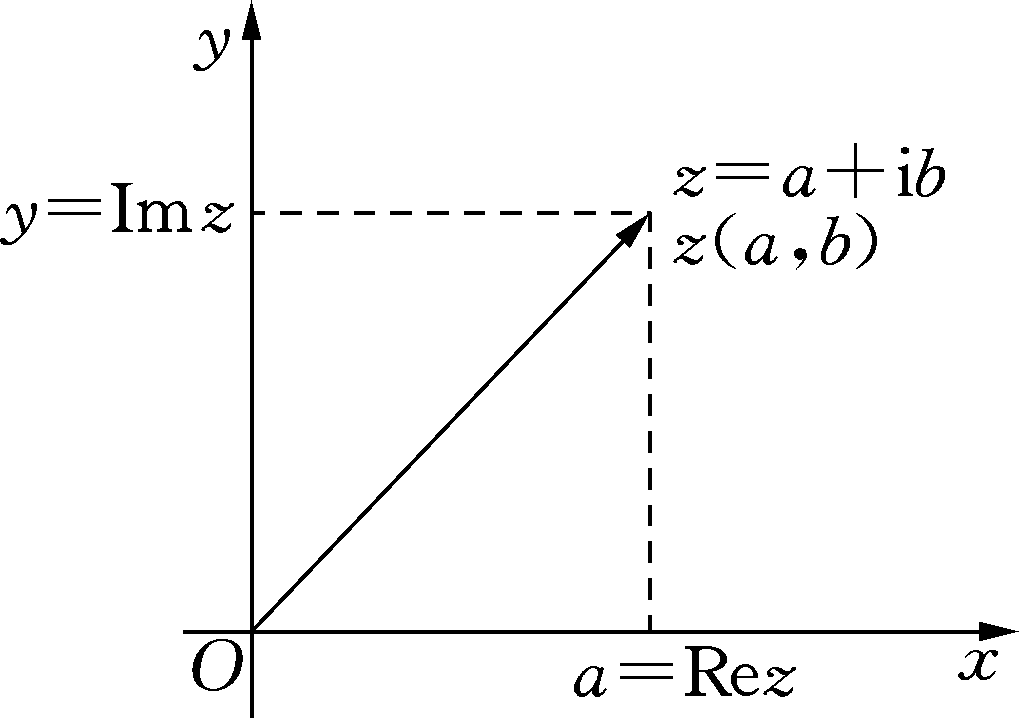
\includegraphics[keepaspectratio,alt={图1.1 复平面与共轭复数}]{figures/01-复数和复平面/fig-p03-c08450d4.png}}
\caption{图1.1 复平面与共轭复数}
\end{figure}

\subsection{1.1.3 复数的模}\label{ux590dux6570ux7684ux6a21}

在复平面上，复数 \(z=a+ib\) 还可用由原点 \(O\) 引向点 \(z\) 的向量
\(\overrightarrow{Oz}\) 表示。该向量的长度称为复数 \(z\)
的\textbf{模}，记作 \(|z|\)（或 \(r\)）：

\[
|z| = r = \sqrt{a^2+b^2} \ge 0 .
\]

模与实部、虚部满足

\[
|\operatorname{Re} z| \le |z| \le |\operatorname{Re} z| + |\operatorname{Im} z|,
\qquad
|\operatorname{Im} z| \le |z| \le |\operatorname{Re} z| + |\operatorname{Im} z| .
\]

\subsection{1.1.4
复数的四则运算}\label{ux590dux6570ux7684ux56dbux5219ux8fd0ux7b97}

设 \(z_1=a+ib\)，\(z_2=c+id\)。

\textbf{加法}

\[
z_1+z_2 = (a+c)+i(b+d).
\]

\textbf{减法}

\[
z_1-z_2 = (a-c)+i(b-d).
\]

\textbf{乘法}

\[
z_1 z_2 = (a+ib)(c+id) = (ac-bd)+i(ad+bc),
\qquad
z^2 = z\cdot z .
\]

\textbf{除法}

\[
\frac{z_1}{z_2}
= \frac{a+ib}{c+id}
= \frac{(a+ib)(c-id)}{(c+id)(c-id)}
= \frac{ac+bd}{c^2+d^2} + i\,\frac{bc-ad}{c^2+d^2},\qquad z_2\neq 0 .
\]

\begin{figure}
\centering
\pandocbounded{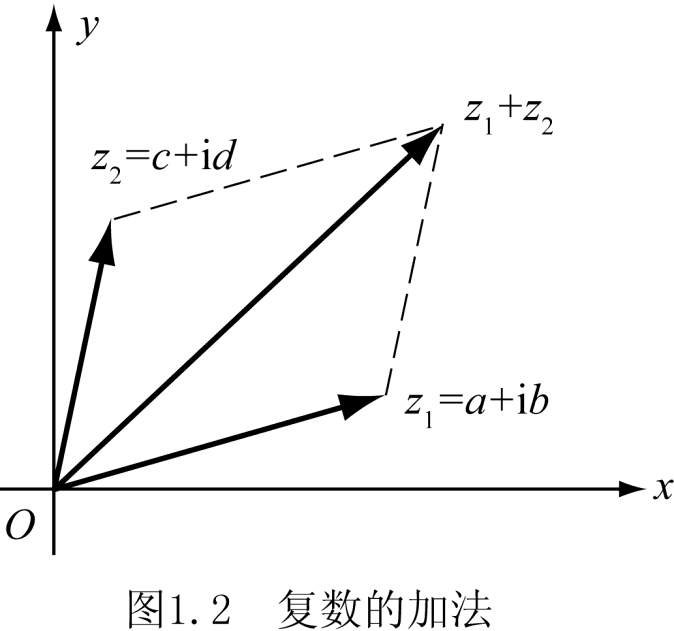
\includegraphics[keepaspectratio,alt={图1.2 复数的加法}]{figures/01-复数和复平面/fig-p04-37af5db3.png}}
\caption{图1.2 复数的加法}
\end{figure}

\subsection{1.1.5
模与共轭复数的性质}\label{ux6a21ux4e0eux5171ux8f6dux590dux6570ux7684ux6027ux8d28}

设 \(z,w \in \mathbb{C}\)，\(w\neq 0\)，则

\[
\begin{aligned}
&(1)\ \operatorname{Re} z = \frac{z+\bar z}{2},\qquad
\operatorname{Im} z = \frac{z-\bar z}{2i};\\[2pt]
&(2)\ \overline{z\pm w} = \bar z \pm \bar w,\qquad
\overline{zw} = \bar z\,\bar w,\qquad
\overline{\left(\frac{z}{w}\right)} = \frac{\bar z}{\bar w};\\[2pt]
&(3)\ z\bar z = |z|^2,\qquad
(4)\ \overline{\bar z} = z,\qquad
(5)\ z+\bar z = 2\operatorname{Re} z,\quad z-\bar z = 2i\operatorname{Im} z .
\end{aligned}
\]

\subsection{1.1.6
复数的三角表示与指数形式}\label{ux590dux6570ux7684ux4e09ux89d2ux8868ux793aux4e0eux6307ux6570ux5f62ux5f0f}

设复平面 \(\mathbb{C}\) 上不为零的点 \(z=x+iy\)，取极坐标

\[
x = r\cos\theta,\qquad y = r\sin\theta,\qquad r=|z| .
\]

\(\theta\) 是正实轴与从原点 \(O\) 到 \(z\) 的射线的夹角，称为复数 \(z\)
的\textbf{辐角}，记作 \(\theta=\operatorname{Arg}z\)。满足

\[
-\pi < \theta \le \pi
\]

的辐角称为 \(\operatorname{Arg}z\) 的\textbf{主值}，记作
\(\theta=\arg z\)，于是

\[
\operatorname{Arg} z = \arg z + 2k\pi,\quad k=0,\pm1,\pm2,\ldots .
\]

复数 \(z\) 有\textbf{三角表示}与\textbf{指数表示}：

\[
z = r(\cos\theta+i\sin\theta)
\qquad\text{与}\qquad
z = re^{i\theta}.
\]

\begin{figure}
\centering
\pandocbounded{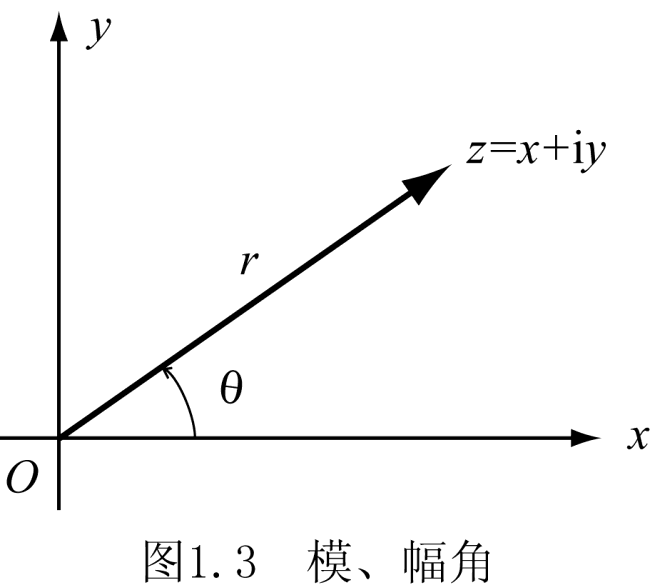
\includegraphics[keepaspectratio,alt={图1.3 极坐标下的复数}]{figures/01-复数和复平面/fig-p06-19f16d72.png}}
\caption{图1.3 极坐标下的复数}
\end{figure}

\textbf{例 1.1} 求 \(\operatorname{Arg}(-3-4i)\)。

\textbf{解} \((-3,-4)\) 位于第三象限，

\[
\arg(-3-4i) = \arctan\frac{4}{3}-\pi,
\]

所以

\[
\operatorname{Arg}(-3-4i)
= \arg(-3-4i)+2k\pi
= \arctan\frac{4}{3} + (2k-1)\pi,
\qquad k=0,\pm1,\pm2,\ldots .
\]

\textbf{例 1.2} 计算 \(z=e^{i\pi}\)。

\textbf{解}

\[
e^{i\pi} = \cos\pi + i\sin\pi = -1 .
\]

\textbf{例 1.3} 把 \(\sqrt3+i\) 表示成三角形式和指数形式。

\textbf{解}
\(r=|\sqrt3+i|=\sqrt{3+1}=2\)，\(\cos\theta=\sqrt3/2\)，点在第一象限，故
\(\theta=\arg(\sqrt3+i)=\pi/6\)，从而

\[
\sqrt3+i = 2\left(\cos\frac{\pi}{6}+i\sin\frac{\pi}{6}\right) = 2e^{i\pi/6}.
\]

\subsection{1.1.7
复数乘除法的几何意义}\label{ux590dux6570ux4e58ux9664ux6cd5ux7684ux51e0ux4f55ux610fux4e49}

设

\[
z_1 = r_1(\cos\theta_1+i\sin\theta_1),\qquad
z_2 = r_2(\cos\theta_2+i\sin\theta_2),
\]

利用三角恒等式可得

\[
\begin{aligned}
z_1z_2
&= r_1r_2\bigl[(\cos\theta_1\cos\theta_2-\sin\theta_1\sin\theta_2)
+i(\sin\theta_1\cos\theta_2+\cos\theta_1\sin\theta_2)\bigr]\\[2pt]
&= r_1r_2\bigl[\cos(\theta_1+\theta_2)+i\sin(\theta_1+\theta_2)\bigr],
\end{aligned}
\]

即

\[
|z_1z_2| = r_1r_2 = |z_1|\,|z_2|,
\qquad
\operatorname{Arg}(z_1z_2) = \operatorname{Arg}z_1+\operatorname{Arg}z_2 .
\]

\textbf{两个复数相乘：积的模等于各复数模的积，积的辐角等于两复数辐角的和。}

类似地，

\[
\left|\frac{z_1}{z_2}\right| = \frac{|z_1|}{|z_2|},
\qquad
\operatorname{Arg}\frac{z_1}{z_2} = \operatorname{Arg}z_1 - \operatorname{Arg}z_2 .
\]

\begin{figure}
\centering
\pandocbounded{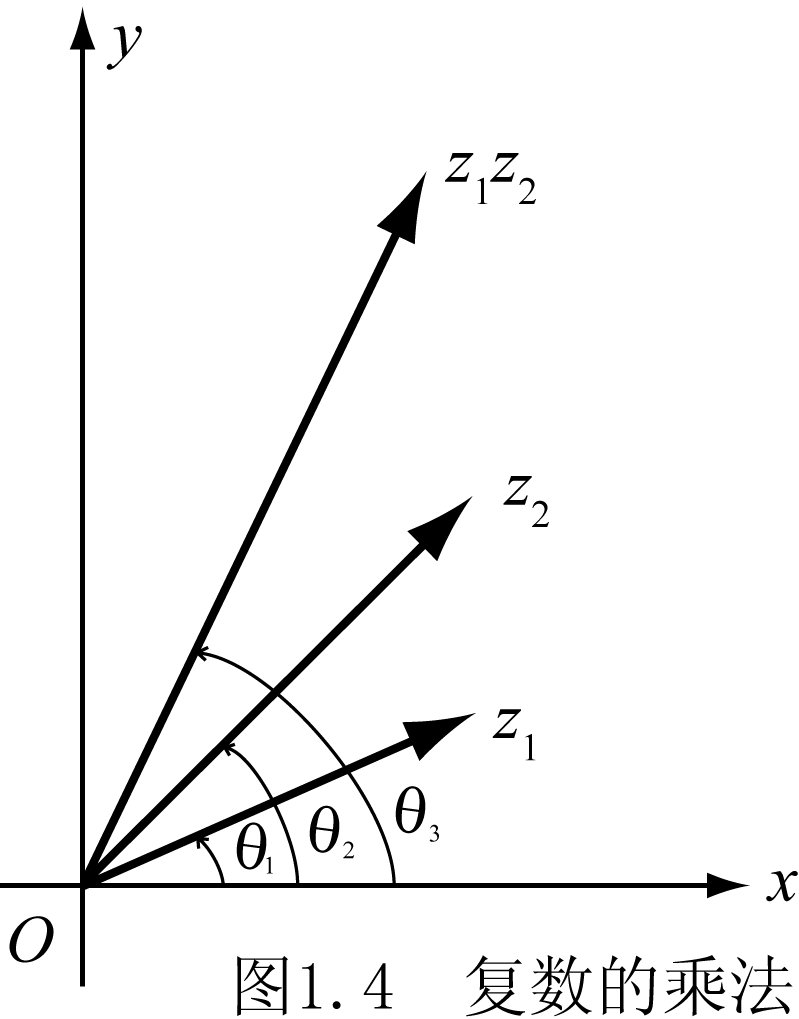
\includegraphics[keepaspectratio,alt={图1.4 复数的乘法}]{figures/01-复数和复平面/fig-p09-23c42b74.png}}
\caption{图1.4 复数的乘法}
\end{figure}

\subsection{1.1.8
复数的乘方与开方}\label{ux590dux6570ux7684ux4e58ux65b9ux4e0eux5f00ux65b9}

\textbf{乘方} 设 \(z=re^{i\theta}\)，则

\[
z^n = \left(re^{i\theta}\right)^n = r^n e^{in\theta}
= r^n(\cos n\theta+i\sin n\theta),
\qquad
|z^n| = |z|^n .
\]

当 \(r=1\) 时，得到 \textbf{棣莫弗（de Moivre）公式}：

\[
(\cos\theta+i\sin\theta)^n = \cos n\theta + i\sin n\theta .
\]

\textbf{开方} 设 \(z=re^{i\theta}\) 是已知复数，\(n\) 为正整数，满足方程

\[
\omega^n = z
\]

的全体复数 \(\omega\) 称为 \(z\) 的 \textbf{\(n\) 次方根}，记作
\(\omega=\sqrt[n]{z}\)。

设 \(\omega=\rho e^{i\varphi}\)，由
\(\rho^n e^{in\varphi}=re^{i\theta}\) 得

\[
\rho = \sqrt[n]{r},\qquad
\varphi = \frac{\theta+2k\pi}{n},\quad k=0,1,\ldots,n-1,
\]

所以

\[
\sqrt[n]{z} = \omega_k
= \sqrt[n]{r}\,e^{i\frac{\theta+2k\pi}{n}},
\qquad k=0,1,2,\ldots,n-1 .
\]

复数的 \(n\) 次方根共有 \(n\) 个：它们的模都等于该复数模的 \(n\)
次算术根，辐角分别等于该复数辐角与 \(0,1,\ldots,n-1\) 倍 \(2\pi\) 之和的
\(n\) 分之一。

\begin{figure}
\centering
\pandocbounded{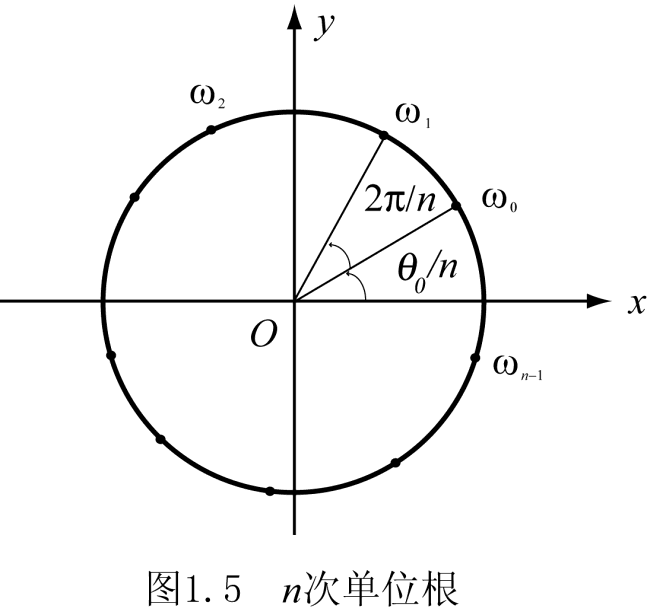
\includegraphics[keepaspectratio,alt={图1.5 n 次方根}]{figures/01-复数和复平面/fig-p12-42098742.png}}
\caption{图1.5 n 次方根}
\end{figure}

\textbf{例 1.4} 求 \(1-i\) 的立方根。

\textbf{解} 先写指数形式：

\[
1-i = \sqrt2\,e^{i7\pi/4},
\]

则

\[
\sqrt[3]{1-i}
= 2^{1/6}e^{i\frac{7\pi/4+2k\pi}{3}}
= 2^{1/6}e^{i\left(\frac{7\pi}{12}+\frac{2k\pi}{3}\right)},
\qquad k=0,1,2 .
\]

即三个立方根为

\[
2^{1/6}e^{i7\pi/12},\qquad
2^{1/6}e^{i5\pi/4},\qquad
2^{1/6}e^{i23\pi/12}.
\]

\textbf{例 1.5} 计算 \(n\) 次单位根。

\textbf{解} \(1=e^{i0}\)，故 \(n\) 次单位根为

\[
1,\quad e^{i\frac{2\pi}{n}},\quad e^{i\frac{4\pi}{n}},\quad \ldots,\quad
e^{i\frac{2(n-1)\pi}{n}} .
\]

立方单位根为

\[
1,\qquad \frac{-1+i\sqrt3}{2},\qquad \frac{-1-i\sqrt3}{2}.
\]

\subsection{常见错误与注意点}\label{ux5e38ux89c1ux9519ux8befux4e0eux6ce8ux610fux70b9}

\begin{enumerate}
\def\labelenumi{\arabic{enumi}.}
\tightlist
\item
  \textbf{辐角是多值的}：\(\operatorname{Arg}z\) 与 \(\arg z\)
  不可混用；写 \(\operatorname{Arg}z\) 时务必补 \(2k\pi\)。
\item
  \textbf{开方记号的约定}：\(\sqrt[n]{z}\) 表示 \(n\)
  个值；实数范围内``根号''的单值约定在复数范围内不再成立。
\item
  \textbf{分母不为零}：作除法 \(z_1/z_2\) 时，必须先说明 \(z_2\neq 0\)。
\item
  \textbf{点 \((a,b)\) vs 向量
  \(\overrightarrow{Oz}\)}：复平面中同一个复数既可看作点，也可看作向量，两者都常用。
\end{enumerate}

\subsection{本节小结}\label{ux672cux8282ux5c0fux7ed3}

\begin{itemize}
\tightlist
\item
  复数 \(z=a+ib\)：实部/虚部、共轭、模、辐角；
\item
  运算：加减乘除、乘方、开方；
\item
  几何意义：乘 = 模相乘 + 辐角相加；除 = 模相除 + 辐角相减；
\item
  工具：三角形式 \(z=r(\cos\theta+i\sin\theta)\) 与指数形式
  \(z=re^{i\theta}\)。
\end{itemize}

\section{1.2 复平面点集}\label{ux590dux5e73ux9762ux70b9ux96c6}

\begin{quote}
本节目标：掌握复平面中的邻域、内点、开集、边界、区域、曲线、连通性等基础概念，会用集合语言描述平面图形。
重点：区域的定义、简单闭曲线、单连通与多连通区域。
难点：直线与半平面的复数表示。
\end{quote}

\subsection{1.2.1
平面点集的几个概念}\label{ux5e73ux9762ux70b9ux96c6ux7684ux51e0ux4e2aux6982ux5ff5}

\textbf{（1）邻域} 集合

\[
D(z_0,\delta) = \{\, z : |z-z_0|<\delta\,\},\qquad \delta>0
\]

称为 \(z_0\) 的 \(\delta\) \textbf{邻域}；而去心邻域为

\[
D(z_0,\delta)\setminus\{z_0\} = \{\, z : 0<|z-z_0|<\delta\,\}.
\]

\textbf{（2）内点、开集} 若点集 \(E\) 的点 \(z_0\) 存在一个邻域
\(D(z_0,\delta)\subset E\)，则称 \(z_0\) 为 \(E\)
的一个\textbf{内点}；若 \(E\) 中的点全为内点，则称 \(E\)
为\textbf{开集}。

\textbf{（3）边界点、边界} 若点 \(z_0\) 的任意邻域内既有属于 \(E\)
的点、又有不属于 \(E\) 的点，则称 \(z_0\) 为 \(E\)
的\textbf{边界点}；\(E\) 的所有边界点组成的集合称为 \(E\)
的\textbf{边界}，记作 \(\partial E\)。

\textbf{（4）区域} 若 \(E\) 内任何两点都可用包含在 \(E\)
内的一条折线连接起来，则称 \(E\)
为\textbf{连通集}。\textbf{连通的开集称为区域}。区域 \(D\) 与其边界
\(\partial D\) 的并集称为\textbf{闭区域}，记为 \(\bar D\)。

\textbf{（5）有界区域} 若存在正数 \(M\)，使得对一切 \(z\in E\) 有
\(|z|\le M\)，则称 \(E\)
为\textbf{有界集}；有界的区域称为\textbf{有界区域}。

\subsection{1.2.2
简单曲线与光滑曲线}\label{ux7b80ux5355ux66f2ux7ebfux4e0eux5149ux6ed1ux66f2ux7ebf}

设 \(x(t)\) 与 \(y(t)\) 是实变量 \(t\) 的两个实函数，在闭区间
\([\alpha,\beta]\) 上连续，则方程组

\[
\begin{cases}
x = x(t),\\
y = y(t),
\end{cases}
\qquad t\in[\alpha,\beta]
\]

或复值函数

\[
z(t) = x(t)+iy(t)
\]

确定的集合称为复平面上的一条\textbf{曲线}，上述方程称为曲线的\textbf{参数方程}。

点 \(A=z(\alpha)\) 与 \(B=z(\beta)\) 分别称为曲线的起点和终点。若当
\(t_1\neq t_2\)（\(t_1,t_2\in[\alpha,\beta]\)）时，\(z(t_1)\neq z(t_2)\)，则称曲线为\textbf{简单曲线}（\textbf{约当
Jordan 曲线}）。若
\(z(\alpha)=z(\beta)\)，则简单曲线称为\textbf{简单闭曲线}。

\textbf{定理 1.1（约当定理）}
一条简单闭曲线把平面分成两个不相交的区域，以该曲线为公共边界。其中一个是有界的，称为曲线的\textbf{内部}；另一个是无界的，称为曲线的\textbf{外部}。

若曲线 \(\Gamma\) 在 \([\alpha,\beta]\) 上 \(x'(t)\)、\(y'(t)\)
存在、连续且不同时为零，则称 \(\Gamma\)
为\textbf{光滑曲线}；由有限条光滑曲线连接而成的连续曲线称为\textbf{分段光滑曲线}。

\subsection{1.2.3
单连通区域与多连通区域}\label{ux5355ux8fdeux901aux533aux57dfux4e0eux591aux8fdeux901aux533aux57df}

\textbf{（7）单连通区域} 设 \(D\) 为复平面上的区域，若 \(D\)
内任意简单闭曲线的内部仍属于 \(D\)，则称 \(D\)
为\textbf{单连通区域}；否则称为\textbf{多连通区域}。

\begin{quote}
直观理解：单连通区域``没有洞''；多连通区域``有洞''（如圆环域）。
\end{quote}

\subsection{1.2.4
直线与半平面}\label{ux76f4ux7ebfux4e0eux534aux5e73ux9762}

设 \(L\) 表示 \(\mathbb{C}\) 中的直线，\(a\) 是 \(L\) 上的任一点，\(b\)
为它的方向向量，则

\[
L = \{\, z : z = a+tb,\ t\in(-\infty,+\infty)\,\}.
\]

对 \(L\) 上的 \(z\)，有

\[
\operatorname{Im}\frac{z-a}{b} = 0 .
\]

由不等式可以定义两个半平面：

\[
L:\ \operatorname{Im}\frac{z-a}{b} = 0,
\qquad
H_0:\ \operatorname{Im}\frac{z-a}{b} > 0,
\qquad
K_0:\ \operatorname{Im}\frac{z-a}{b} < 0 .
\]

为方便，假定 \(|b|=1\) 且 \(a=0\)。令
\(b=e^{i\beta}\)，\(z=re^{i\theta}\)，则

\[
\frac{z}{b} = re^{i(\theta-\beta)},
\]

于是 \(z\in H_0\) 当且仅当 \(\operatorname{Im}\frac{z}{b}>0\)，即

\[
\sin(\theta-\beta)>0
\quad\Longleftrightarrow\quad
\beta<\theta<\beta+\pi .
\]

若``按 \(b\) 的方向沿 \(L\) 前进''，则 \(H_0\) 是位于 \(L\)
\textbf{左边}的半平面；由平移可得

\[
H_a = \{\, w : w=a+h,\ h\in H_0\,\} = \left\{\,z : \operatorname{Im}\frac{z-a}{b}>0\,\right\}
\]

是位于 \(L\) 左边的半平面，而

\[
K_a = \left\{\,z : \operatorname{Im}\frac{z-a}{b}<0\,\right\}
\]

是位于 \(L\) 右边的半平面。

\subsection{常见错误与注意点}\label{ux5e38ux89c1ux9519ux8befux4e0eux6ce8ux610fux70b9-1}

\begin{enumerate}
\def\labelenumi{\arabic{enumi}.}
\tightlist
\item
  ``连通的开集是区域''是标准定义；不要漏掉``开集''这一条件。
\item
  边界点不要求属于集合本身：闭区域 \(\bar D=D\cup\partial D\) 包含边界。
\item
  简单曲线可以自交？不可以；简单曲线要求不同的参数对应不同的点。
\item
  半平面的判别式 \(\operatorname{Im}\frac{z-a}{b}\) 的正负与方向向量
  \(b\) 的选择有关。
\end{enumerate}

\subsection{本节小结}\label{ux672cux8282ux5c0fux7ed3-1}

\begin{itemize}
\tightlist
\item
  邻域、内点、开集、边界、区域、闭区域、有界区域；
\item
  曲线、简单曲线、简单闭曲线、光滑曲线、分段光滑曲线；
\item
  约当定理：简单闭曲线划分内部与外部；
\item
  单连通/多连通区域；
\item
  直线与半平面：\(\operatorname{Im}\frac{z-a}{b}\gtrless 0\)。
\end{itemize}

\section{1.3
扩充复平面及其球面表示}\label{ux6269ux5145ux590dux5e73ux9762ux53caux5176ux7403ux9762ux8868ux793a}

\begin{quote}
本节目标：理解无穷远点 \(\infty\)
的引入方式、扩充复平面的运算约定以及球面（黎曼球面）表示。
重点：扩充复平面 \(\mathbb{C}_\infty\)；无穷远点的球面模型。
难点：为什么无穷远点只有一个；哪些运算不规定意义。
\end{quote}

\subsection{1.3.1
扩充复平面的运算约定}\label{ux6269ux5145ux590dux5e73ux9762ux7684ux8fd0ux7b97ux7ea6ux5b9a}

设 \(a\) 是异于 \(\infty\) 的一个复数，规定：

\[
\begin{aligned}
&(1)\ a\neq\infty \ \Rightarrow\ a\pm\infty = \infty\pm a = \infty;\\[2pt]
&(2)\ a\neq 0 \ \Rightarrow\ a\cdot\infty = \infty\cdot a = \infty;\\[2pt]
&(3)\ a\neq\infty \ \Rightarrow\ \frac{a}{\infty}=0,\qquad
a\neq 0 \ \Rightarrow\ \frac{\infty}{a}=\infty .
\end{aligned}
\]

\(\infty\)
的实部、虚部、辐角都无意义。为了避免与算术定律矛盾，对下列式子\textbf{不规定意义}：

\[
\infty\pm\infty,\qquad \infty\cdot 0,\qquad 0\cdot\infty,\qquad \frac{0}{\infty},\qquad \frac{\infty}{\infty},\qquad \frac{\infty}{0}.
\]

\subsection{1.3.2 扩充复平面}\label{ux6269ux5145ux590dux5e73ux9762}

设想平面上有一个``理想点''与 \(\infty\)
对应，称为\textbf{无穷远点}。复平面加上
\(\infty\)，称为\textbf{扩充复平面}：

\[
\mathbb{C}_\infty = \mathbb{C}\cup\{\infty\}.
\]

为使运算法则合理，规定\textbf{扩充复平面上只有一个无穷远点}。

\subsection{1.3.3
球面表示（黎曼球面）}\label{ux7403ux9762ux8868ux793aux9eceux66fcux7403ux9762}

记 \(\mathbb{R}^3\) 中的单位球面为

\[
S = \{(x_1,x_2,x_3): x_1^2+x_2^2+x_3^2=1\},
\qquad N=(0,0,1)\ \text{为北极点}.
\]

把复平面 \(\mathbb{C}\) 等同于 \(\mathbb{R}^3\) 中的点集

\[
\{(x_1,x_2,0): x_1,x_2\in\mathbb{R}\}.
\]

对复平面内任意一点 \(z\)，用直线将 \(z\) 与北极点 \(N\)
相连，该直线与球面 \(S\) 恰交于一点
\(Z\neq N\)。这个对应给出复平面到``去北极点的球面''的一一映射，称为\textbf{球面投影（stereographic
projection）}。

\begin{itemize}
\tightlist
\item
  若 \(|z|>1\)，则 \(Z\) 位于北半球面上；
\item
  若 \(|z|<1\)，则 \(Z\) 位于南半球面上；
\item
  若 \(|z|=1\)，则 \(Z=z\)；
\item
  当 \(|z|\to\infty\) 时，\(Z\to N\)。
\end{itemize}

于是\textbf{扩充复平面 \(\mathbb{C}_\infty\) 与整个球面 \(S\)（含北极点
\(N\)）一一对应}；北极点 \(N\) 正好对应无穷远点
\(\infty\)。这一模型称为\textbf{黎曼球面}。

\subsection{常见错误与注意点}\label{ux5e38ux89c1ux9519ux8befux4e0eux6ce8ux610fux70b9-2}

\begin{enumerate}
\def\labelenumi{\arabic{enumi}.}
\tightlist
\item
  \(\infty\)
  只有一个：复平面不是``四面八方无穷远''，而是``一个无穷远点''。
\item
  不能把 \(\infty\)
  当成普通复数参与四则运算；\(\infty\pm\infty\)、\(\infty\cdot 0\)
  等均不定义。
\item
  球面投影中，\(|z|\) 越大越接近北极，但不等于``正无穷''有多个方向。
\end{enumerate}

\subsection{本节小结}\label{ux672cux8282ux5c0fux7ed3-2}

\begin{itemize}
\tightlist
\item
  \(\mathbb{C}_\infty=\mathbb{C}\cup\{\infty\}\)；
\item
  无穷远点的运算约定与禁用式；
\item
  黎曼球面：复平面去掉一点（北极点）与球面同胚，\(z\to\infty\)
  对应北极点。
\end{itemize}

\section{第1章
本章小结与教学建议}\label{ux7b2c1ux7ae0-ux672cux7ae0ux5c0fux7ed3ux4e0eux6559ux5b66ux5efaux8bae}

\subsection{知识框架}\label{ux77e5ux8bc6ux6846ux67b6}

\begin{enumerate}
\def\labelenumi{\arabic{enumi}.}
\tightlist
\item
  复数：概念、相等、共轭、模、辐角（主值）、三角形式、指数形式；
\item
  运算：加减乘除、乘方（棣莫弗公式）、开方（n 个 n 次方根）；
\item
  几何：复平面上的点/向量表示，乘除法的模与辐角规律；
\item
  点集语言：邻域、内点、开集、边界、区域、闭区域、有界、曲线、单连通；
\item
  扩充复平面：\(\mathbb{C}_\infty = \mathbb{C}\cup\{\infty\}\)，黎曼球面模型。
\end{enumerate}

\subsection{教学建议}\label{ux6559ux5b66ux5efaux8bae}

\begin{itemize}
\tightlist
\item
  第1节宜慢讲：学生的困惑主要在``辐角的多值性''和``\(z\)
  既是点又是向量''；
\item
  乘除法的几何意义建议配合图形（复平面上的向量加法和乘法图）讲解；
\item
  开方一节可与后续``解析函数的多值性''呼应；
\item
  点集概念是第2、3章的基础，建议把``区域''与``单连通''作为重点，多举例（圆盘、圆环、去心圆盘、半平面）；
\item
  球面表示可作为选讲内容，帮助理解 \(\infty\)。
\end{itemize}

\subsection{常见考点提示}\label{ux5e38ux89c1ux8003ux70b9ux63d0ux793a}

\begin{itemize}
\tightlist
\item
  已知 \(z\)，求
  \(\operatorname{Re}z,\operatorname{Im}z,|z|,\bar z,\operatorname{Arg}z\)；
\item
  将复数化为三角/指数形式；
\item
  求 \(n\) 次方根、\(n\) 次单位根；
\item
  判断平面图形（圆、圆环、角域、半平面等）并写出集合表达式；
\item
  判断区域是否单连通。
\end{itemize}

\newpage
